\section{Architettura} \label{section:architettura}

Per lo sviluppo generale dell'applicazione, è stata seguita una architettura DApp, (Fully) Decentralised Application.
Essa consiste in un frontend Web che effettua chiamate dirette ad una infrastruttura decentralizzata backend, nel 
nostro caso una gerarchia di smartcontracts eseguiti su blockchain Fantom; 
questa struttura ricorda quindi una architettura client-server, senza un supporto intermedio per le operazioni.
\\
\\
Il pattern architetturale scelto dal gruppo per lo sviluppo del frontend è il Model-View-ViewModel. Il
seguente pattern è tra i più diffusi nello sviluppo delle web application e permette di scrivere codice
facilmente mantenibile e riusabile; questo è possibile grazie al forte disaccoppiamento che sussiste tra
logica di presentazione e di business. Inoltre l'MVVM è risultato il più adatto per essere utilizzato con
React, libreria impiegata per lo sviluppo dell'UI e che renderizza le componenti in base al loro stato
interno.

\begin{figure}[H]
    \centering
    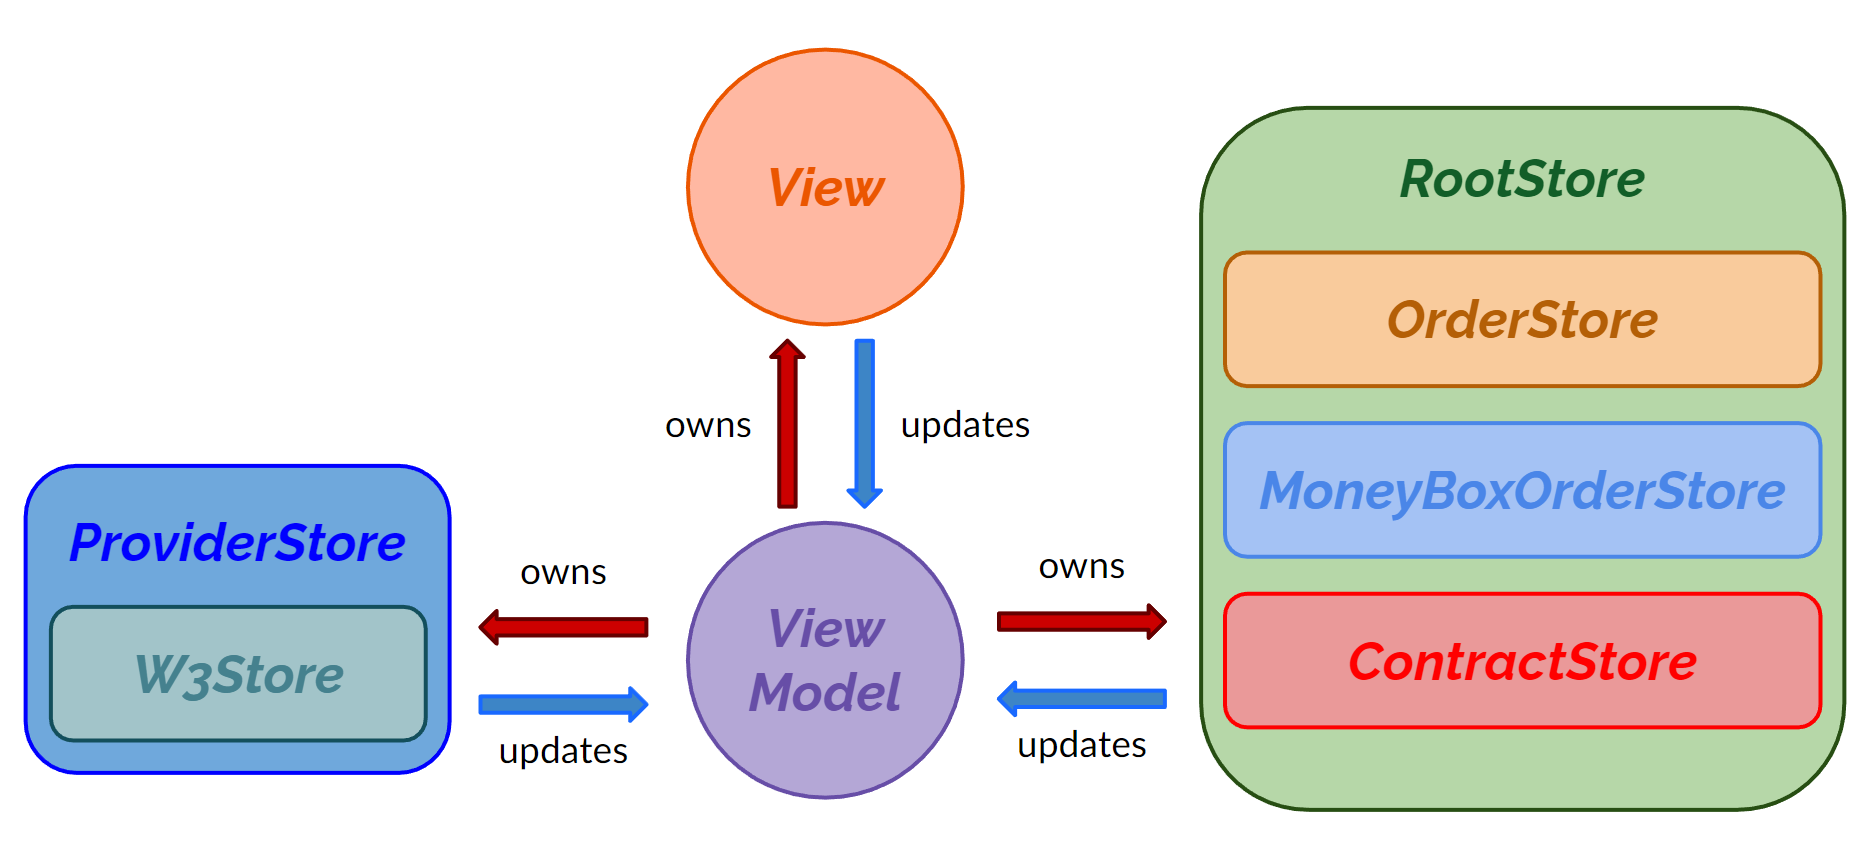
\includegraphics[scale=0.3]{immagini/mvvm.png}
    \caption{Model-View-ViewModel di ShopChain}
\end{figure}

Il passaggio dei dati dal Model alle varie componenti grafiche avviene attraverso l'utilizzo di un Context
React, al quale viene passato un'istanza del ViewModel. L'utilizzo di un Context React ci permette di
accedere al valore corrente del ViewModel in qualsiasi porzione della View, senza doverlo passare di
componente in componente attraverso le props (ossia gli argomenti dei componenti che compongono la
vista). Nella radice dell'applicazione viene infatti creata un'istanza del ViewModel, che viene passata
ad un Context.Provider, che fa da contenitore per tutta la View. All'interno di tale contenitore ogni
componente puo' utilizzare un hook per accedere al Context React ed utilizzare il valore più recente del ViewModel.
\\
\\
E' stato scelto di utilizzare un Context React per il passaggio dei dati in quanto la nostra applicazione è
molto profonda e non risultava conveniente passare i dati per molti componenti rischiando, nel peggiore
dei casi, di doverli utilizzare nell'ultimo della gerarchia.
Per poter fare in modo che una componente della View si renderizzi non solo al cambiamento del
suo stato interno ma anche al cambiamento dei dati nel Model, abbiamo utilizzato la libreria Mobx.
Questa ci permette di implementare l'observer pattern, non supportato di default da React. A tale
scopo, Mobx permette di segnare delle classi (o attributi di esse) come "observable" e di costruire
dei componenti della View come "observer". Quest'ultimi vengono automaticamente ri-renderizzati al
cambiamento di un qualsiasi attributo observable.